% 't Hooft and Wilson defects in 2+1d BF theory: Hopf-linked line operators.
% The BF action (N/2pi) int B wedge dA gives linking phase exp(2pi i/N)
% when the Wilson line W (sourcing A) links the 't Hooft line T (sourcing B).
\begin{tikzpicture}[scale=1.3, thick,
    wilson/.style={very thick, blue!70!black},
    thooft/.style={very thick, red!65!black},
    field A/.style={blue!40!black, thin, dashed, ->, >=stealth},
    field B/.style={red!40!black, thin, dotted, ->, >=stealth},
    faded/.style={opacity=0.25}]

  % === Wilson line W (electric, couples to A): horizontal ellipse ===
  % Center at origin, radii 2.2 x 0.8

  % Back arc of W (behind T)
  \draw[wilson, faded] (180:2.2 and 0.8) arc (180:360:2.2 and 0.8);

  % Front arc of W
  \draw[wilson] (180:2.2 and 0.8) arc (180:0:2.2 and 0.8);

  % Orientation arrow on W
  \draw[blue!70!black, ->, >=stealth, line width=1pt]
    (70:2.2 and 0.8) -- (65:2.2 and 0.8);

  % === 't Hooft line T (magnetic, couples to B): vertical ellipse ===
  % Center at (0.4, 0), radii 0.8 x 1.8, oriented in the xz-plane.
  % T threads through W, forming a Hopf link.

  % Back arc of T (below W's plane)
  \draw[thooft, faded]
    (-0.15, 0.0)
    .. controls (-0.35, -0.8) and (0.0, -1.6) .. (0.5, -1.8)
    .. controls (1.0, -1.6) and (1.35, -0.8) .. (1.15, 0.0);

  % White knockout where T crosses over W on the right
  \draw[white, line width=6pt]
    (1.1, 0.2) -- (1.15, 0.0) -- (1.12, -0.15);

  % Front arc of T (above W's plane)
  \draw[thooft]
    (-0.15, 0.0)
    .. controls (-0.25, 0.8) and (0.05, 1.55) .. (0.5, 1.75)
    .. controls (0.95, 1.55) and (1.2, 0.8) .. (1.15, 0.0);

  % Orientation arrow on T
  \draw[red!65!black, ->, >=stealth, line width=1pt]
    (0.0, 1.1) -- (0.12, 1.25);

  % === Field lines: A-field radiating from W ===
  \draw[field A] (-1.8, 0.55) -- ++(-0.5, 0.3);
  \draw[field A] (-1.6, -0.5) -- ++(-0.5, -0.2);
  \draw[field A] (1.9, -0.5) -- ++(0.5, -0.2);

  % === Field lines: B-field radiating from T ===
  \draw[field B] (0.5, 1.75) -- ++(0.0, 0.5);
  \draw[field B] (-0.3, -1.35) -- ++(-0.4, -0.35);
  \draw[field B] (1.1, -1.5) -- ++(0.4, -0.3);

  % === Piercing points (where T threads through W's disk) ===
  \fill[red!80!black] (-0.15, 0.0) circle (2pt);
  \fill[red!80!black] (1.15, 0.0) circle (2pt);

  % === Labels ===
  % Wilson line
  \node[blue!70!black, font=\small, anchor=east] at (-2.5, 0.4)
    {$W$ \textrm{\footnotesize (electric)}};
  \node[blue!40!black, font=\scriptsize, anchor=east] at (-2.5, -0.6)
    {$A$-field};

  % 't Hooft line
  \node[red!65!black, font=\small] at (0.5, -2.15)
    {$T$ \textrm{\footnotesize (magnetic)}};
  \node[red!40!black, font=\scriptsize, anchor=south] at (0.5, 2.35)
    {$B$-field};

  % Linking phase annotation
  \node[font=\footnotesize, gray, anchor=north west, align=left] at (3.0, 1.4)
    {$\displaystyle \langle W \cdot T \rangle \;=\; e^{2\pi i/N}$\\[6pt]
     \footnotesize $S_{\mathrm{BF}} = \dfrac{N}{2\pi}\displaystyle\int B \wedge F$\\[8pt]
     \footnotesize $\mathrm{Lk}(W, T) = +1$};

  % Spacetime dimension
  \node[font=\scriptsize, gray, anchor=north] at (0.3, -2.7)
    {2+1d: both $W$, $T$ are line operators};

\end{tikzpicture}
